\documentclass[11pt,a4paper]{article}
\usepackage[utf8]{inputenc}
\usepackage[T1]{fontenc}
\usepackage{lmodern}
\usepackage{textcomp}
\usepackage{amsmath,amssymb,amsthm}
\usepackage{booktabs,array}
\usepackage{enumitem}
\usepackage{xcolor}
\usepackage[expansion=false]{microtype}
\usepackage{url}
\usepackage{graphicx}
\usepackage[margin=2.6cm]{geometry}
\usepackage[pdftitle={Rado numbers of a(x-y)=bz with a<b},pdfauthor={Takumi Ichikawa},colorlinks=true,linkcolor=blue!50!black,citecolor=blue!50!black,urlcolor=blue!50!black]{hyperref}

\newtheorem{theorem}{Theorem}[section]
\newtheorem{lemma}[theorem]{Lemma}
\newtheorem{proposition}[theorem]{Proposition}
\newtheorem{corollary}[theorem]{Corollary}
\newtheorem{conjecture}[theorem]{Conjecture}
\theoremstyle{definition}
\newtheorem{definition}[theorem]{Definition}
\theoremstyle{remark}
\newtheorem{remark}[theorem]{Remark}

\newcommand{\R}{\mathrm{R}}
\newcommand{\todo}[1]{\textcolor{red}{[#1]}}
\setlist{itemsep=2pt,topsep=4pt}
\allowdisplaybreaks

\title{Rado numbers of $a(x-y)=bz$ with $a<b$:\\[4pt]
\large two colours, lower bounds for every number of colours,\\
and the three-colour upper bound up to one statement}
\author{Takumi Ichikawa\\ \small\texttt{github.com/IchiTaku326}}
\date{Version 2, 4 November 2026\\ \small (preprint, not peer reviewed; version 1: 3 November 2026)}

\begin{document}
\maketitle

\begin{abstract}
For coprime integers $2\le a<b$ let $\R_k(a,b)$ be the least $n$ such that every $k$-colouring of $\{1,\dots,n\}$ contains a monochromatic solution of $a(x-y)=bz$.
We prove the following.
\begin{enumerate}[label=(\arabic*),leftmargin=2em,itemsep=1pt,topsep=2pt]
\item The extremal $2$-colouring for $\R_2(a,b)=b^2+b+1$ (a value conjectured by Gasarch, Moriarty and Tumma and proved by Yao) is unique; this gives a new proof of the value.
\item $\R_3(a,b)\ge N(a,b)$ for all $a<b$, by one explicit colouring; here $N(a,b)=b(b^2+b+2a+1)+1$ when $a^2+(b-1)a\le b^2+b+1$, and $N$ is given by a short formula otherwise.
\item $\R_3(a,a+1)=a^3+5a^2+8a$ for all $a\ge7$; the upper bound is a symbolic SAT certificate checked by a formally verified checker.
\item $\R_k(a,b)>b^k$ for all $k$ and all $a<b$, by a recursive colouring in the spirit of the Schur product construction; a refined recursion gives $\R_k(a,b)\ge L_k$ for every $k$, where $L_2=b^2+b+1$ and $L_k=b(L_{k-1}+2a)+1$, whenever $a/b\le(\sqrt5-1)/2$; more precisely, in the region of~(2) the construction works for all $k$ exactly when $D=a^2+ab-b^2$ satisfies $D\le1$ or $a+1\le D\le2a$.
\item The upper bound $\R_3(a,b)\le N(a,b)$ follows from a single statement (Conjecture~S) about the colours of the multiples of $a$; we prove this reduction, prove that Conjecture~S follows from its restriction to the multiples $am$ with $m\le\max(ab+4a,4b)$, and verify that restriction by computer for all pairs with $b\le30$ in the main region except $(2,3)$ and $(2,5)$. Conjecture~S itself remains open.
\end{enumerate}
Finally, $\R_3=N$ (with the two exceptions $(2,3)$ and $(2,5)$) is verified with checked proofs for all $b\le60$; this confirms Conjecture~1.1 of Ahmed, Zaman and Bright in that range. A common thread is the quantity $D=a^2+ab-b^2$, the norm of $a+b\phi$ in $\mathbb Z[\phi]$, $\phi=(1+\sqrt5)/2$: it decides the shape of the three-colour formula and the range of the recursion for every number of colours.
\end{abstract}

{\setcounter{tocdepth}{1}\small
\makeatletter\renewcommand{\l@section}{\@dottedtocline{1}{0em}{1.5em}}\makeatother
\renewcommand{\contentsname}{\normalsize Contents}%
\tableofcontents}
\clearpage

%======================================================================
\section{Introduction}
%======================================================================

\subsection{The problem}
For positive integers $a,b$ and $k$, the \emph{Rado number} $\R_k(a,b)$ is the least $n$ such that every colouring of $[n]=\{1,\dots,n\}$ with $k$ colours contains a \emph{monochromatic solution} of
\[
  a(x-y)=bz ,
\]
that is, positive integers $x,y,z\le n$ of the same colour (not necessarily distinct) satisfying the equation. Rado's theorem \cite{Rado33} implies that this equation is regular (the coefficients $a$ and $-a$ sum to zero), so $\R_k(a,b)$ is finite for every $k$. A colouring of $[n]$ without monochromatic solution is called \emph{good}.

Throughout, $\gcd(a,b)=1$. Then every solution has the form
\begin{equation}\label{eq:sol}
  z=as,\qquad x-y=bs\qquad(s\ge1),
\end{equation}
and $x\equiv y\pmod a$ holds if and only if $a\mid s$. We use these two facts without further mention.

\subsection{Known results}
\begin{itemize}
\item $\R_1(a,b)=\max(a,b+1)$.
\item Two colours: Gasarch, Moriarty and Tumma \cite[Theorem~3.3]{GMT12} proved $\R_2(a,b)\ge b^2+b+1$ for $a\le b$ and conjectured equality \cite[Conjecture~3.4]{GMT12}; Yao \cite{Yao14} proved the conjecture for $1<a<b$.
\item Three colours, $a>b$: Chang, De Loera and Wesley \cite{CDW22} proved $\R_3=a^3$ for $a\ge b+2$ and $\R_3=a^3+(a-1)^2$ for $a=b+1$, using symbolic SAT certificates.
\item Three colours, $a<b$: Ahmed, Zaman and Bright \cite{AZB25} write the equation as $ax+by=bz$ (the letters $a,b$ exchanged). In our notation they proved $\R_3\ge b(b^2+b+2a+1)+1$ when $b^2+b+a>a^2+ab$, and conjectured equality for $a\ge3$ \cite[Theorem~1.3 and Conjecture~1.1]{AZB25}.
\item Four colours: in a previous note we computed $\R_4(2,3)=226$ \cite{Ich26a}; a companion note \cite{Ich26b} gives further four-colour values.
\item Many colours: Sanders \cite{San26} proved $\R_k(a,b)\le\exp\bigl(k^{2+o(1)}\bigr)$ (see Section~\ref{sec:rec}).
\end{itemize}

\subsection{Notation}
We write $\R_2=b^2+b+1$ (this is justified by Theorem~\ref{thm:R2}) and
\begin{align*}
  M &= b\,(b^2+b+a+1)=b\,(\R_2+a), \\
  A &= \{\,au'+bu \;:\; 1\le u,u'\le b\,\}, \\
  m' &= \min\{\,m\in A \;:\; am>M\,\}\qquad(\text{$m'=\infty$ if there is no such $m$}),\\
  N(a,b) &= \min\bigl(am',\; M+ab+1\bigr).
\end{align*}
We call $a^2+(b-1)a\le b^2+b+1$ the \emph{main region}. In the main region no element of $A$ exceeds $M/a$, so
\[
  N(a,b)=M+ab+1=b\,(\R_2+2a)+1=b(b^2+b+2a+1)+1 .
\]
This is the value of \cite{AZB25}; their condition $b^2+b+a>a^2+ab$ is the same as ours. Roughly, the main region is $a\le0.618\,b$. We also use
\[
  D=a^2+ab-b^2,\qquad L_2=b^2+b+1,\qquad L_k=b\,(L_{k-1}+2a)+1\quad(k\ge3).
\]
Note $L_3=N(a,b)$ in the main region, and $D\le0$ iff $a/b\le(\sqrt5-1)/2$ (the ``golden-ratio region'').

\subsection{Results}
\begin{theorem}[two colours; the value is due to Yao \cite{Yao14}]\label{thm:R2}
Let $2\le a<b$ and $\gcd(a,b)=1$. Then $\R_2(a,b)=b^2+b+1$. Moreover, if $(a,b)\ne(2,3)$, the only good $2$-colouring of $[b(b+1)]$ (up to swapping the colours) gives
\[
  Q=\{a,2a,\dots,ab\}
\]
one colour and all other numbers the other colour.
\end{theorem}

\begin{theorem}[three colours, lower bound]\label{thm:lower}
For all $2\le a<b$ with $\gcd(a,b)=1$: $\ \R_3(a,b)\ge N(a,b)$.
\end{theorem}

\begin{theorem}[the family $b=a+1$]\label{thm:j1}
For all $a\ge7$: $\ \R_3\bigl(a(x-y)=(a+1)z\bigr)=a^3+5a^2+8a$.
\end{theorem}

\begin{theorem}[every number of colours]\label{thm:R}
\begin{enumerate}[label=(\alph*)]
\item For all $2\le a<b$ and $k\ge2$: $\R_k(a,b)\ge L'_k$, where $L'_2=b^2+b+1$ and $L'_k=b\,(L'_{k-1}+a)+1$. In particular $\R_k(a,b)>b^k$.
\item If $a^2+ab\le b^2$, then $\R_k(a,b)\ge L_k$ for every $k\ge2$. In the main region, the recursive colouring of Section~\ref{sec:rec} proves $\R_k\ge L_k$ for all $k$ if and only if $D\le1$ or $a+1\le D\le2a$ (Theorem~\ref{thm:D}).
\end{enumerate}
\end{theorem}

\begin{conjecture}\label{conj:C3}
$\R_3(a,b)=N(a,b)$ for all $2\le a<b$ with $\gcd(a,b)=1$, except $(a,b)=(2,3)$ and $(2,5)$, where $\R_3=61$ and $181$.
\end{conjecture}

\begin{theorem}[reduction of the upper bound]\label{thm:red}
Let $(a,b)\ne(2,3)$ and $a\nmid M$; if $(a,b)$ is outside the main region assume also $b\ge a+2$. If Conjecture~S (Section~\ref{sec:upper}) holds for $(a,b)$, then $\R_3(a,b)\le N(a,b)$, and hence $\R_3(a,b)=N(a,b)$.
\end{theorem}

\begin{table}[ht]
\centering
\small
\renewcommand{\arraystretch}{1.1}
\begin{tabular}{>{\raggedright}p{6.2cm}>{\raggedright\arraybackslash}p{7.4cm}}
\toprule
Statement & Status\\
\midrule
$\R_2=b^2+b+1$ & known \cite{Yao14}; new proof (Theorem~\ref{thm:R2})\\
unique extremal $2$-colouring & proved (Theorem~\ref{thm:R2})\\
$\R_3\ge N(a,b)$ & proved (Theorem~\ref{thm:lower})\\
$\R_3(a,a+1)=a^3+5a^2+8a$, $a\ge7$ & proved (Theorem~\ref{thm:j1}; computer-assisted)\\
$\R_k\ge L'_k>b^k$ for all $k$ & proved for all $a<b$ (Theorem~\ref{thm:R}(a))\\
$\R_k\ge L_k$ for all $k$ & proved for $D\le1$ or $a+1\le D\le 2a$ (Theorems~\ref{thm:R}, \ref{thm:D})\\
$\R_3\le N(a,b)$ & follows from Conjecture~S (Theorem~\ref{thm:red})\\
Conjecture~S & follows from its lower part (Theorem~\ref{thm:upind}); lower part checked by SAT solver for $b\le30$ (Section~\ref{sec:lowerpart}); open in general\\
$\R_3=N(a,b)$, $b\le60$ & checked proofs (Section~\ref{sec:comp}), except $(2,3)$, $(2,5)$\\
$\R_3=N(a,b)$, $b\le81$ & SAT solver (Section~\ref{sec:comp}), except $(2,3)$, $(2,5)$\\
\bottomrule
\end{tabular}
\caption{Summary of the results on $a(x-y)=bz$, $2\le a<b$, $\gcd(a,b)=1$.}
\end{table}

Theorem~\ref{thm:lower} contains the lower bound of \cite{AZB25} and extends it to all $a<b$. The family of Theorem~\ref{thm:j1} lies outside the range of their conjecture. Conjecture~\ref{conj:C3} holds for all $1939$ pairs with $b\le81$, and for $b\le60$ the upper bounds come with checked proofs.

\paragraph{Organisation.} Section~\ref{sec:R2} proves the two-colour theorem, Section~\ref{sec:lower} the three-colour lower bound, and Section~\ref{sec:rec} the recursive construction for every $k$. Section~\ref{sec:small} explains the small set used for computer proofs of upper bounds, Section~\ref{sec:j1} the family $b=a+1$, and Section~\ref{sec:upper} the reduction of the upper bound to Conjecture~S and of Conjecture~S to its lower part. Section~\ref{sec:comp} lists the computations, and Section~\ref{sec:open} collects what we could not prove.

%======================================================================
\clearpage
\section{Two colours}\label{sec:R2}
%======================================================================
In this section $n=b(b+1)$. A solution in $[n]$ has $x-y=bs\le n-1<b(b+1)$, so $s\le b$ and $z=as\in Q$.

\begin{proof}[Proof of Theorem~\ref{thm:R2}]
Let $\chi:[n]\to\{A,B\}$ be a good colouring with $\chi(1)=A$, and put
\[
  g(u)=\chi(au)\ \ (1\le u\le b),\qquad G_A=\{u:g(u)=A\},\qquad G_B=\{u:g(u)=B\}.
\]
\emph{Classes.} For $r\in[1,b]$ the \emph{class} of $r$ consists of the $b+1$ numbers $r,r+b,\dots,r+b^2$; the number $r+ib$ has \emph{index} $i\in[0,b]$. Two numbers of the same class with index difference $d$ form a solution with $z=ad$. Hence:
\begin{equation}\label{eq:class}
  \text{if two numbers of one class have colour $c$ and index difference $d$, then } g(d)\ne c .
\end{equation}
The number $au$ ($1\le u\le b$) lies in the class of $au\bmod b$ at index $k(u)=\lfloor(au-1)/b\rfloor\le a-1$, and different $u$ give different classes. The class of $1$ contains $1$ (index $0$) and $au_0$, where $au_0\equiv1\pmod b$, $1\le u_0\le b-1$, at index $k(u_0)\in[1,a-1]$.

\emph{Counting.} Fix a class and let $S$, $S'$ be the sets of indices of colour $A$ and $B$. By \eqref{eq:class}, all differences inside $S$ lie in $G_B$, and all differences inside $S'$ lie in $G_A$. Measuring from the smallest element we get $|S|\le|G_B|+1$ and $|S'|\le|G_A|+1$, while
\[
  |S|+|S'|=b+1=|G_A|+|G_B|+1 .
\]
So in every class at least one of the two inequalities is an equality; we say that $S$ (or $S'$) is \emph{tight}. If $S$ is tight, then $S-\min S=\{0\}\cup G_B$, and since this set contains all differences of its elements, it is closed under taking positive differences. A finite set of integers containing $0$ with this property is an arithmetic progression $\{0,d,2d,\dots\}$. So
\[
  \text{$S$ tight}\ \Longrightarrow\ G_B=\{d,2d,\dots,\ell d\}\ \text{for some $d,\ell$};\qquad
  \text{$S'$ tight}\ \Longrightarrow\ G_A=\{e,2e,\dots,\ell'e\}.
\]

\emph{Case analysis.}
\begin{enumerate}[label=(\alph*)]
\item $G_B=\emptyset$. Then every class contains at most one number of colour $A$. But the class of $1$ contains $1$ and $au_0$, and $g(u_0)=A$. Impossible.
\item $G_A=\emptyset$. Then every class contains at most one number of colour $B$, and every $au$ has colour $B$. Since the $au$ lie in distinct classes, the numbers of colour $B$ are exactly the elements of $Q$. This is the colouring of the theorem.
\item $G_A,G_B$ both non-empty, and $S$ is tight in some class and $S'$ in another. Then both $G_A$ and $G_B$ are arithmetic progressions starting at their common difference, and they partition $[1,b]$. This forces $\{G_A,G_B\}=\{[1,b-1],\{b\}\}$.
  \begin{itemize}
  \item If $G_A=\{b\}$: in every class the indices of colour $B$ have all differences equal to $b$, so they are a single index or $\{0,b\}$. The number $au$ ($u\le b-1$) has colour $B$ and index $k(u)\le a-1<b$, so $k(u)=0$ for all $u\le b-1$, i.e.\ $a(b-1)\le b$. This is false for $a\ge2$, $b\ge3$.
  \item If $G_B=\{b\}$: in the class of $1$, the indices of colour $A$ include $0$ and $k(u_0)\in[1,a-1]$, with difference not equal to $b$. Impossible.
  \end{itemize}
\item $G_A,G_B$ non-empty and $S$ tight in every class. Then $G_B=\{d,\dots,\ell d\}$, and in the class of $1$ (where index $0$ has colour $A$) we get $S=\{0,d,\dots,\ell d\}$.
  If $d=b$ we are in case (c). If $d=1$, the indices of colour $B$ in that class form an interval in which no difference $1$ is allowed, so a single index; then $G_A\subseteq\{b\}$, case (c). If $2\le d<b$, the indices $1$ and $d+1$ both have colour $B$ and difference $d\in G_B$, contradicting \eqref{eq:class}.
\item $G_A,G_B$ non-empty and $S'$ tight in every class. Then $G_A=\{e,\dots,\ell'e\}$.
  If $e\ge2$: in the class of $1$ the index $e$ cannot be $A$ (difference $e\in G_A$ from index $0$), so it is $B$, and the $B$-indices are $\{e,2e,\dots\}$; then indices $1$ and $1+e$ are both $A$ with difference $e\in G_A$. Impossible.
  If $e=1$: $G_A=[1,\ell']$, the $B$-indices of every class form an interval, and each of the two end pieces of colour $A$ has at most one index; hence $\ell'\ge b-2$. In the class of $1$ the $B$-interval is $[1,\ell'+1]$ and contains $k(u_0)$, so $u_0\in G_B\subseteq\{b-1,b\}$, hence $u_0=b-1$, i.e.\ $a\equiv-1\pmod b$, i.e.\ $a=b-1$. Then $2a=2b-2$ lies at index $1$ of its class and $g(2)=A$ (as $2\le \ell'$ when $b\ge4$); but index $1$ is neither an end of the interval of $B$'s nor allowed to be $B$. Impossible, except for $b=3$, i.e.\ $(a,b)=(2,3)$.
\end{enumerate}
This proves the uniqueness statement.

\emph{The value.} The colouring of the theorem is good \cite{GMT12}, so $\R_2\ge b^2+b+1$. Let $n_2=b^2+b+1$ and suppose $\chi$ is a good colouring of $[n_2]$. For $(a,b)=(2,3)$ a direct computation gives $\R_2=13$; otherwise the restriction of $\chi$ to $[b(b+1)]$ is the colouring above, with $Q$ coloured $B$.
\begin{itemize}
\item If $\chi(n_2)=A$: then $(n_2,1,a(b+1))$ is a solution, and $a(b+1)\notin Q$ has colour $A$, as does $1$.
\item If $\chi(n_2)=B$: take $t_0\in[1,a-1]$ with $bt_0+1\equiv0\pmod a$ and $s=b+1-t_0\in[1,b]$. Then $y=n_2-bs=bt_0+1$ is a multiple of $a$ at most $ab$, so $y\in Q$; also $z=as\in Q$. So $(n_2,y,z)$ is a solution of colour $B$.
\end{itemize}
In both cases there is a monochromatic solution, so $\R_2\le n_2$.
\end{proof}
We also checked the uniqueness by computer for all $450$ pairs with $b\le40$. The value $\R_2=b^2+b+1$ for $1<a<b$ was first proved by Yao \cite{Yao14}; our contribution in this section is the uniqueness of the extremal colouring, which we need in Section~\ref{sec:upper}, and with it a short proof of the value.

%======================================================================
\clearpage
\section{The three-colour lower bound}\label{sec:lower}
%======================================================================
\begin{proof}[Proof of Theorem~\ref{thm:lower}]
Put $n=N-1$. By the definition of $N$ we have $n\le M+ab$, and no $m\in A$ satisfies $M<am\le n$.
Let $Q_2=\{a^2u:1\le u\le b\}$ and colour $[n]$ by
\begin{align*}
C_0&=\{x\le ab-1:\ a\nmid x\}\ \cup\ Q_2\ \cup\ [M+1,n],\\
C_1&=\{x\le ab(b+1):\ a\mid x\}\setminus C_0,\\
C_2&=\{ab+1\le x\le M:\ a\nmid x\}\ \cup\ \{ab(b+1)<x\le M:\ a\mid x\}.
\end{align*}
These sets partition $[n]$, because $a^2b<M$ and $ab(b+1)<M$. Let $(x,y,z)$ be a monochromatic solution, $z=as$, $x-y=bs$, $x>y$. Recall $x\equiv y\pmod a$ iff $a\mid s$, i.e.\ iff $a^2\mid z$.
\begin{enumerate}[label=(\roman*)]
\item $z\in C_1$. Then $x,y\in C_1$ are multiples of $a$, so $a^2\mid z$; as $z\notin Q_2$, $z=a^2t$ with $t>b$. Then $x-y=abt\ge ab(b+1)\ge\max C_1$. Impossible.
\item $z\in C_2$. Then $z$ is a multiple of $a$, so $z>ab(b+1)$ and $s\ge b^2+b+1$. Hence $x\ge\min C_2+bs\ge ab+1+b^3+b^2+b=M+1>\max C_2$. Impossible.
\item $z\in[M+1,n]$. Then $x>bz/a\ge b(M+1)/a$, and
\[
  b(M+1)-a(M+ab)=(b-a)M-b(a^2-1)>0
\]
since $M>b^3>a^2b$. So $x>n$. Impossible.
\item $z\in Q_2$, $z=a^2u$ with $u\le b$. Then $x-y=abu\ge ab$ and $x\equiv y\pmod a$.
  \begin{itemize}
  \item If $y\le ab-1$ and $a\nmid y$: then $a\nmid x$ and $ab+1\le x\le ab-1+ab^2\le M$, so $x\in C_2$.
  \item If $y=a^2u'\in Q_2$: then $x=a(au'+bu)=am$ with $m\in A$. Now $x\in Q_2$ would force $a\mid u$ and then $x\ge a^2(b+1)>\max Q_2$; and $x\in[M+1,n]$ contradicts the choice of $N$.
  \item If $y\ge M+1$: then $x-y\le n-M-1<ab$. \qedhere
  \end{itemize}
\end{enumerate}
\end{proof}

\begin{remark}
In the main region the colouring is the case $k=3$ of the recursive colouring of Section~\ref{sec:rec}. Outside the main region the last block $[M+1,n]$ is shorter: it stops just below the first ``dangerous'' multiple $am'$, $m'\in A$. When $a\mid M$ the value $N=am'$ can be very close to $M$; for $b\le100$ there are $14$ such pairs.
\end{remark}

\subsection{The formula in terms of \texorpdfstring{$D$}{D}}\label{sec:NinD}
The value $N(a,b)$ is governed by the same quantity $D=a^2+ab-b^2$ that controls the recursion in Section~\ref{sec:rec}. Put
\[
  E=D-(a+b+1),\qquad
  \sigma(x)=\max\{\,ai+bj:\ i,j\ge0,\ ai+bj<x\,\}\quad(x>0),
\]
so $\sigma$ only depends on the numerical semigroup generated by $a$ and $b$.
\begin{proposition}\label{prop:NinD}
The main region is exactly $E\le0$, i.e.\ $D\le a+b+1$, and there $N=b(b^2+b+2a+1)+1$. If $E>0$, then
\[
  N(a,b)=\min\Bigl(M+ab+1,\ a\bigl(b(a+b)-\sigma(bE/a)\bigr)\Bigr).
\]
\end{proposition}
\begin{proof}
Writing $u'=b-i$, $u=b-j$ with $0\le i,j\le b-1$ we get $A=\{\,b(a+b)-(ai+bj)\,\}$. A direct computation gives
\[
  a\cdot b(a+b)-M=b\,(D-a-b-1)=bE ,
\]
so $am>M$ for $m=b(a+b)-(ai+bj)$ iff $ai+bj<bE/a$. If $E\le0$ there is no such $m$; this is the main region, since $a^2+(b-1)a\le b^2+b+1$ is equivalent to $E\le0$. If $E>0$, the least such $m$ is $b(a+b)-\sigma(bE/a)$; the restriction $i,j\le b-1$ is harmless because $bE/a<b(a+b)$ and every value of $ai+bj$ below $b(a+b)$ can be written with $i,j\le b-1$ after replacing $ai$ by $a(i-b)+ba$ when $i\ge b$.
\end{proof}
By computer, outside the main region the minimum is always the second term (all pairs with $b\le200$), so there $N=a\,(b(a+b)-\sigma(bE/a))$: the value is the largest possible dangerous multiple $ab(a+b)$, lowered by the largest element of the semigroup $\langle a,b\rangle$ below $bE/a$. In particular $N=ab(a+b)$ exactly when $0<bE/a\le a$, which explains the pairs with $\R_3=ab(a+b)$ observed in our tables. So the whole three-colour formula is a function of the norm $D=\mathrm N(a+b\phi)$ (Section~\ref{sec:norm}) and of the semigroup $\langle a,b\rangle$.

\paragraph{The staircase outside the main region.} Put $x=bE/a$ and $F=ab-a-b$ (the Frobenius number of $\langle a,b\rangle$). Since $M=ab(a+b)-bE$, one has $a\lceil (M+1)/a\rceil=a\bigl(b(a+b)-\lceil x\rceil+1\bigr)$, and Proposition~\ref{prop:NinD} becomes
\[
  N(a,b)=a\Bigl\lceil\frac{M+1}{a}\Bigr\rceil+a\,\delta,\qquad
  \delta=\bigl(\lceil x\rceil-1\bigr)-\sigma(x)\ \ge0 .
\]
So $\delta$ is the distance from $\lceil x\rceil-1$ down to the semigroup $\langle a,b\rangle$: $\delta=0$ (the ``unified'' value $a\lceil(M+1)/a\rceil$, the least multiple of $a$ above $M$) whenever $\lceil x\rceil-1$ is representable as $ai+bj$, and $\delta>0$ exactly when $\lceil x\rceil-1$ is a gap of the semigroup. For $0<x\le a$ we are on the plateau $N=ab(a+b)$. Writing $\rho=a/b$, we have $x\approx (D/a^2)\,F$ with $D/a^2=1+1/\rho-1/\rho^2$, which vanishes at $\rho=1/\phi$ and tends to $1$ as $\rho\to1$. Since the proportion of gaps of $\langle a,b\rangle$ near height $\theta F$ is roughly $1-\theta$, one expects the proportion of pairs with $\delta>0$ near a given ratio $\rho$ to be about $1-D/a^2=(1-\rho)/\rho^2$. The data agree well:
\begin{center}
\small
\begin{tabular}{lcccccccc}
\toprule
$a/b\approx$ & $0.66$ & $0.70$ & $0.74$ & $0.78$ & $0.82$ & $0.86$ & $0.90$ & $0.94$\\
\midrule
observed share with $\delta>0$ & $0.85$ & $0.62$ & $0.44$ & $0.41$ & $0.27$ & $0.19$ & $0.13$ & $0.08$\\
$(1-\rho)/\rho^2$ & $0.78$ & $0.61$ & $0.47$ & $0.36$ & $0.27$ & $0.19$ & $0.12$ & $0.07$\\
\bottomrule
\end{tabular}
\end{center}
(all pairs outside the main region with $b\le240$, grouped by $a/b$). Thus the irregular ``staircase'' of values just outside the main region is the gap structure of the numerical semigroup $\langle a,b\rangle$, read at the height $D/a^2$ given by the norm; it thins out as $a/b\to1$.

%======================================================================
\clearpage
\section{A recursive construction for every number of colours}\label{sec:rec}
%======================================================================

\subsection{One step of the recursion}
\begin{lemma}\label{lem:step}
Let $k\ge3$, $L\ge2$, and let $C'$ be a good $(k-1)$-colouring of $[1,L-1]$ with colours $0,\dots,k-2$ such that
\begin{enumerate}[label=(I\arabic*)]
\item all numbers of colour $1$ are multiples of $a$, and
\item no number $am+bs$ with $C'(m)=C'(s)=1$ lies in the interval $(M_k,n_k]$, where
\[
  M_k=b\,(L+a),\qquad n_k=b\,(L+2a).
\]
\end{enumerate}
Let $\sigma$ swap the colours $0$ and $1$ and fix the others. Colour $[1,n_k]$ with $k$ colours as follows.
\begin{center}
\renewcommand{\arraystretch}{1.15}
\begin{tabular}{lll}
\toprule
number & range & colour\\
\midrule
$a\nmid x$ & $x\le ab-1$ & $0$\\
 & $ab<x\le M_k$ & $k-1$\\
 & $x>M_k$ & $0$\\
\midrule
$x=am$ & $m\le L-1$ & $\sigma(C'(m))$\\
 & $m\ge L$ and $x\le M_k$ & $k-1$\\
 & $x>M_k$ & $0$\\
\bottomrule
\end{tabular}
\end{center}
This colouring is good and again satisfies (I1). Hence $\R_k\ge b(L+2a)+1$.
\end{lemma}
\begin{proof}
The ``copy'' $a\cdot[1,L-1]$ lies below $M_k$ (as $a<b$). Colours $1,\dots,k-2$ occur only in the copy, colour $k-1$ only in $[ab+1,M_k]$, and colour $0$ on $\{x\le ab-1:a\nmid x\}$, on $\{am:C'(m)=1\}$ and on $(M_k,n_k]$. Let $(x,y,z)$ be a monochromatic solution, $z=as$, $x-y=bs$, $x>y$.
\begin{enumerate}[label=(\roman*)]
\item $z$ has colour $k-1$. Then $s\ge L$ and $x-y\ge bL$, but colour $k-1$ lies in an interval of length $M_k-ab-1<bL$. Impossible.
\item $z$ has colour $c\in[1,k-2]$. Then $x,y$ are in the copy, and $(x/a,y/a,s)$ is a monochromatic solution for $C'$. Impossible.
\item $z\in(M_k,n_k]$. Then $x>bz/a\ge b(M_k+1)/a>n_k$, since $b(M_k+1)-an_k=bL(b-a)+b(ab+1-2a^2)>0$ (if $b\ge2a$ the second term is non-negative; otherwise $L(b-a)\ge L\ge b^2>a(2a-b)$).
\item $z$ is in the copy and has colour $0$. Then $C'(s)=1$, so $a\mid s$ by (I1), $x-y\ge ab$ and $x\equiv y\pmod a$.
  \begin{itemize}
  \item If $y\le ab-1$, $a\nmid y$: then $a\nmid x$ and $ab<x<M_k$, so $x$ has colour $k-1$.
  \item If $y=aY$ with $C'(Y)=1$: if $x$ is in the copy, $(x/a,Y,s)$ is a monochromatic solution for $C'$; otherwise $x=a(Y+bs/a)=aY+bs\in(M_k,n_k]$, which (I2) excludes.
  \item If $y>M_k$: then $x-y<ab$. \qedhere
  \end{itemize}
\end{enumerate}
\end{proof}

\begin{corollary}[without (I2)]\label{cor:noI2}
If $C'$ satisfies (I1) but not necessarily (I2), the colouring of Lemma~\ref{lem:step} restricted to $[1,M_k]$ is still good and satisfies (I1). Hence $\R_k\ge b(L+a)+1$.
\end{corollary}
\begin{proof}
In the proof of Lemma~\ref{lem:step}, (I2) was used only when $x\in(M_k,n_k]$, which does not occur in $[1,M_k]$; all other cases are unchanged.
\end{proof}
\begin{proof}[Proof of Theorem~\ref{thm:R}(a)]
Start with $T_2$ (which satisfies (I1)) and apply Corollary~\ref{cor:noI2} repeatedly. Since $L'_k>bL'_{k-1}$ and $L'_2>b^2$, we get $L'_k>b^k$.
\end{proof}
The same corollary can be applied to any good colouring with (I1), for instance to the colouring of Theorem~\ref{thm:lower}: $\R_4(a,b)\ge b\,(N(a,b)+a)+1$ for all $a<b$. We checked the colourings of Theorem~\ref{thm:R}(a) against all solutions for all pairs with $b\le12$ and $k=3,4$.

\paragraph{Growth in $k$.} Theorem~\ref{thm:R}(a) is the analogue of the classical product construction for Schur numbers, $S(k+1)\ge3S(k)+1$: a colouring with $k-1$ colours is copied (here: multiplied by $a$), and one new colour fills a long block. It shows that $\R_k(a,b)$ grows at least like $b^k$. For every coprime pair the colouring of $[a^k-1]$ by the exponent $v_a(x)$ of $a$ in $x$ is good: a monochromatic solution would have $v_a(x)=v_a(y)=v_a(z)=j$, but $z=as$ and $x-y=bs$ give $v_a(x-y)=v_a(s)=j-1<j$. So $\R_k(a,b)\ge a^k$ always; this is \cite[Lemma~4.1]{CDW22}, where also $\R_3=a^3$ is proved for $a\ge b+2$. Together with Theorem~\ref{thm:R}(a):
\[
  \liminf_{k\to\infty}\R_k(a,b)^{1/k}\ \ge\ \max(a,b)\qquad\text{for all coprime }a,b\ge2 .
\]
It is natural to ask:
\begin{conjecture}[question]\label{conj:growth}
For coprime $a,b\ge2$, $a\ne b$: is $\ \lim_{k\to\infty}\R_k(a,b)^{1/k}=\max(a,b)$?
\end{conjecture}
So only the upper half is open. For the Schur equation $x-y=z$ ($a=b=1$) the growth rate is not known; the best bounds are roughly $3.28^k\lesssim S(k)\le e\,k!$. For $a\ne b$ the coefficients seem to determine it. The known four-colour values agree: $\R_4=a^4$ for $(a,b)=(3,1),(4,1),(5,1)$ \cite[Table~10]{CDW22} and $(5,2),(5,3)$ (with checked proofs, \cite{Ich26b}), and $\R_4(3,4)=461\approx1.80\cdot4^4$. However, the exact formula $\R_k=a^k$ does not persist: we found a good $5$-colouring of $[243]$ for $3(x-y)=z$ (checked against all solutions), so $\R_5\bigl(3(x-y)=z\bigr)>243=3^5$. In fact $\R_5\bigl(3(x-y)=z\bigr)>320$ (an explicit colouring of $[320]$, checked; in all good $5$-colourings we found, the numbers with $v_3(x)=1$ form one colour class), so the ratio $\R_5/\R_4$ is at least $3.95$ for $3(x-y)=z$, compared with $\R_2/\R_1=\R_3/\R_2=\R_4/\R_3=3$. Similarly for $3(x-y)=2z$ the ratios are $\R_3/\R_2=3.44$, $\R_4/\R_3=3.32$ and $\R_5/\R_4\ge3.87$ (from $\R_4=103$ and $\R_5\ge399$, an explicit colouring of $[398]$, checked against all solutions), and for $4(x-y)=3z$ we have $\R_4=313$ and $\R_5\ge1401$ \cite{Ich26b}, so $\R_5/\R_4\ge4.47>4$. These ratios do not yet decrease towards $3$, so the answer to the question above may well be negative for $a>b$; the data are too few to decide. The best general upper bound we know is due to Sanders \cite{San26}, who proved $\R_k(a,b)\le\exp\bigl(k^{2+o(1)}\bigr)$ for fixed $a,b$ (for the equation $ax-ay=bz$, i.e.\ exactly our family); we know no upper bound of the form $C^k$.

\paragraph{Density.} Each colour class is a solution-free set, and such sets can be very large.
\begin{proposition}\label{prop:density}
Let $2\le a<b$, $\gcd(a,b)=1$, $n\ge1$ and $S=\lfloor(n-1)/b\rfloor$. The set $[n]\setminus\{a,2a,\dots,aS\}$ contains no solution. If $b\ge4$, every solution-free subset of $[n]$ has at most $n-S$ elements.
\end{proposition}
\begin{proof}
\emph{Construction.} A solution has $z=as$ with $bs=x-y\le n-1$, i.e.\ $s\le S$; so $z$ is one of the removed numbers.

\emph{Upper bound.} Let $A\subseteq[n]$ be solution-free; we show that at least $S$ numbers are missing from $A$. If $as\notin A$ for all $s\le S$, we are done. Otherwise let $g$ be the least $s\le S$ with $ag\in A$. Then $a,2a,\dots,a(g-1)$ are missing, and since $z=ag\in A$, the set $A$ contains no two numbers at distance $d=bg$.
\begin{itemize}
\item If $d\le n-2S$: the graph on $[n]$ joining $x$ and $x+d$ is a union of $\min(d,n)$ paths with $n$ vertices in total, and a set without an edge misses at least $\lfloor L/2\rfloor$ vertices of a path with $L$ vertices. Hence at least $(n-d)/2\ge S$ numbers are missing.
\item If $d>n-2S$: since $b\ge4$ we have $2S<n/2$, so $d>n/2$ and the pairs $\{y,y+d\}$, $1\le y\le n-d$, are disjoint. Each pair contains a missing number. The larger number $y+d>d>a(g-1)$ is never one of $a,\dots,a(g-1)$, and at most $\lfloor(n-d)/a\rfloor$ of the smaller numbers are. So at least
\[
  (g-1)+(n-d)-\Bigl\lfloor\frac{n-d}{a}\Bigr\rfloor\ \ge\ (g-1)+\Bigl\lceil\frac{(n-d)(a-1)}{a}\Bigr\rceil
\]
numbers are missing. As $n-d\ge b(S-g)+1$ and $b(a-1)/a\ge1$, this is at least $(g-1)+(S-g)+1=S$. \qedhere
\end{itemize}
\end{proof}
For $(a,b)=(2,3)$ the same maximum $n-S$ holds for all $n\le60$ by computer. So a single colour class can cover a proportion $1-1/b$ of $[n]$. Since the coefficients $a,-a,-b$ do not sum to zero, this is the ``non-invariant'' case of Ruzsa's theory \cite{Ruz93}, where solution-free sets have positive density; density arguments therefore give no useful upper bound on $\R_k$, and the Rado numbers are governed by structure (the copy and the blocks) rather than by density.

\subsection{The colourings \texorpdfstring{$T_k$}{T\_k}}
Let $T_2$ be the colouring of Theorem~\ref{thm:R2} on $[1,L_2-1]$, with $Q$ coloured $1$; it satisfies (I1). Applying Lemma~\ref{lem:step} repeatedly (as long as (I2) holds) gives good colourings $T_k$ of $[1,L_k-1]$. The colouring $T_3$ is the colouring of Theorem~\ref{thm:lower} in the main region, and (I2) at $k=3$ is exactly the main-region condition.

\begin{proof}[Proof of Theorem~\ref{thm:R} for $a^2+ab\le b^2$]
The colour-$1$ numbers of $T_{k-1}$ are at most $a(L_{k-2}-1)$, so every sum $am+bs$ in (I2) is less than
\[
  a(a+b)L_{k-2}\ \le\ b^2L_{k-2}\ <\ bL_{k-1}\ <\ M_k. \qedhere
\]
\end{proof}

Write $C_c^{(k)}$ for the set of numbers of colour $c$ in $T_k$ and $N_{ab}=\{x<ab:\ a\nmid x\}$. The table in Lemma~\ref{lem:step} gives
\begin{equation}\label{eq:recsets}
  C_0^{(k)}=N_{ab}\cup J_k\cup aC_1^{(k-1)},\qquad C_1^{(k)}=aC_0^{(k-1)},\qquad J_k=(M_k,L_k-1].
\end{equation}
In particular every $C_c^{(k)}$ is a union of $O(ka)$ arithmetic progressions, so (I2) can be decided exactly by computer even when $L_k$ is huge.

\subsection{When does the recursion work?}
\begin{theorem}\label{thm:D}
Assume the main region, i.e.\ $D\le a+b+1$. Condition (I2) holds at every step $k\ge3$ (so $\R_k\ge L_k$ for all $k$) if and only if
\[
  D\le1\qquad\text{or}\qquad a+1\le D\le2a .
\]
More precisely: (I2) first fails at $k=4$ if $D\ge2a+1$, first fails at $k=5$ if $2\le D\le a$, and never fails otherwise.
\end{theorem}

\begin{proof}
For $D\le0$ this is the proof of Theorem~\ref{thm:R}. Let $D\ge1$. Then $a<b<2a$ and $x:=a/b\in(0.618,\,0.76)$. At step $k$ the relevant set is $C=C_1^{(k-1)}$, and we put $X=L_{k-2}$. We will use
\[
  M_k=b^2X+2ab^2+ab+b,\qquad L_{k-2}>b^2L_{k-4}.
\]
For $k\ge5$, \eqref{eq:recsets} gives $C=I\cup R$, where the \emph{top block} $I=aJ_{k-2}$ is $a$ times an interval of length $ab$, and the \emph{rest} $R=aN_{ab}\cup a^2C_1^{(k-3)}$ satisfies $\max R<a^3L_{k-4}$ (for $k=5$: $\max R=a^3b$). The \emph{window} is $(M_k,M_k+ab]$.

\medskip\noindent\emph{Step $k=4$.} Here $C=C_1^{(3)}=aC_0^{(2)}$ with $C_0^{(2)}=[1,b(b+1)]\setminus Q$. The sums are $a(ax+by)$ with $x,y\in C_0^{(2)}$, the largest being $aT$ with $T=(a+b)(b^2+b)$. A direct computation gives
\[
  aT-M_4=b\,\bigl[(b+1)(D-2a-1)+a\bigr].
\]
If $D\le2a$ this is negative, and no sum reaches the window. If $D\ge2a+1$, the window corresponds to $b$ consecutive values of $ax+by$ just below $T$; they contain a value $T-ai$ with $i\ge0$, obtained from $x=b^2+b-i$ (which is $>ab$, hence in $C_0^{(2)}$) and $y=b^2+b$. So (I2) fails.

\medskip\noindent\emph{Step $k=5$, both numbers in $I$.} The sums are $at$ with
\[
  t\in t_{\min}+\{ai+bj:\ 0\le i,j<ab\}.
\]
This set contains $t_{\min}+ai$ and $t_{\max}-ai$ for all $0\le i<ab$; hence $b>a$ consecutive values of $t$ between $t_{\min}$ and $t_{\max}$ always meet it. The window lies inside $[at_{\min},at_{\max}]$ iff both of the following are positive:
\begin{align*}
  M_5-a(a+b)(M_3+1) &= -D\,(b^3+b^2+b+1+ab)+b\,\bigl(a(b+1)^2+1\bigr),\\
  a(a+b)(L_3-1)-M_5 &= b\,\bigl[D\,(b^2+b+1+2a)-(2ab+a+b+1)\bigr].
\end{align*}
The first is positive for $D\le a$ and less than $-ab$ for $D\ge a+1$ (its zero lies strictly between $a$ and $a+1$). The second is positive for $D\ge2$ and negative for $D=1$. So these sums hit the window iff $2\le D\le a$.

\medskip\noindent\emph{Steps $k\ge6$, both numbers in $I$.} The smallest sum is $a(a+b)(X-ab)$, and
\[
  a(a+b)(X-ab)-(M_k+ab)=DX-a^2b(a+b)-2ab^2-2ab-b>0,
\]
because $DX\ge L_4=b^4+b^3+b^2+2ab^2+b+2ab+1$ and $a^2(a+b)\le a(b^2+a+b+1)$ (main region).

\medskip\noindent\emph{Steps $k\ge5$, other pairs.} Write $\{s,m\}$ for the two numbers, the sum being $am+bs$.
\begin{itemize}
\item $s\in I$, $m\in R$: $am+bs<a^4L_{k-4}+ab(X-1)$ and $M_k-ab(X-1)>(b-a)bX>(b-a)b^3L_{k-4}$. This is at least $a^4L_{k-4}$ when $x^4+x\le1$, i.e.\ $x\le0.724$. In the main region with $D\ge1$ this holds except for $(a,b)=(3,4)$, treated below.
\item $m\in I$, $s\in R$: $am+bs<a^2X+a^3X/b\le b^2X$, since $x^2+x^3\le1$.
\item $m,s\in R$: $am+bs<(a+b)a^3X/b^2\le b^2X$, since $x^3(1+x)\le1$.
\end{itemize}
For $k=5$ the same estimates hold with $L_{k-4}$ replaced by $b$ and $X=L_3>b^3$.

\medskip\noindent\emph{The pair $(3,4)$ with $s\in I$, $m\in R$.} Here $X=16L'+125$ with $L'=L_{k-4}$, and $M_k=16X+112$. For $k=5,6$ we check directly: $am\le324$, resp.\ $am\le1620$, both below $M_k-ab(X-1)$. For $k\ge7$ split $R$ further. If $m\in a^3J_{k-4}$, the sums are at least $12(X-12)+81(L'-12)=273L'+384>256L'+2124=M_k+ab$, since $L'\ge109$. For the remaining $m\in a^4C_1^{(k-5)}\cup a^3N_{ab}\cup aN_{ab}$ we have $am<46L'$ and the sums are less than $12X+46L'<M_k$.
\end{proof}

We confirmed Theorem~\ref{thm:D} by an exact computation of (I2) using \eqref{eq:recsets}: all main-region pairs with $b\le120$ and $k\le20$, with $b\le40$ and $k\le60$, and with $b\le250$ and $k\le6$. Examples: $(5,7)$ ($D=11=2a+1$) fails at $k=4$; $(7,11)$ ($D=5$) fails at $k=5$; $(3,4)$ ($D=5$) and consecutive Fibonacci numbers such as $(5,8)$, $(13,21)$ ($D=1$) work for all $k$. In particular $\R_4(3,4)\ge461$ and $\R_5(3,4)\ge1869$; the first bound is sharp \cite{Ich26b}.

\subsection{The golden-ratio field}\label{sec:norm}
The quantity $D$ has a natural meaning. Let $\phi=(1+\sqrt5)/2$ and $\bar\phi=(1-\sqrt5)/2=-1/\phi$. In the ring $\mathbb Z[\phi]$ the norm of $a+b\phi$ is
\[
  \mathrm{N}(a+b\phi)=(a+b\phi)(a+b\bar\phi)=a^2+ab-b^2=D .
\]
Since $a+b\bar\phi=a-b/\phi$, this gives the exact identity
\begin{equation}\label{eq:t}
  t:=a-\frac b\phi=\frac{D}{a+b\phi}.
\end{equation}
So $D$ measures how far the line $a=b/\phi$ is from the point $(a,b)$, and all conditions in this paper are, up to a correction of order $1/b$, conditions on $t$. Using $a\approx b/\phi$, so that $a+b\phi\approx b\sqrt5$, \eqref{eq:t} turns the conditions on $D$ into the following picture.
\begin{center}
\renewcommand{\arraystretch}{1.2}
\small
\begin{tabular}{ll>{\raggedright\arraybackslash}p{5.4cm}}
\toprule
condition on $D$ & condition on $t=a-b/\phi$ (approx.) & meaning\\
\midrule
$D\le0$ & $t\le0$ & golden-ratio region; recursion works for all $k$\\
$D=1$ & $t\approx 1/(b\sqrt5)$ & consecutive Fibonacci numbers: works for all $k$\\
$2\le D\le a$ & $0<t\lesssim 1/(\phi\sqrt5)\approx0.276$ & (I2) first fails at $k=5$\\
$a+1\le D\le 2a$ & $0.276\lesssim t\lesssim 2/(\phi\sqrt5)\approx0.553$ & works for all $k$\\
$2a+1\le D\le a+b+1$ & $0.553\lesssim t\lesssim \phi/\sqrt5\approx0.724$ & (I2) first fails at $k=4$\\
$D>a+b+1$ & $t\gtrsim0.724$ & outside the main region\\
\bottomrule
\end{tabular}
\end{center}
For all $11618$ main-region pairs with $b\le250$ the observed ranges of $t$ in the five classes are disjoint, except that the five Fibonacci pairs lie inside the range of the class ``$2\le D\le a$'': the Fibonacci exception is arithmetic, not metric. In particular the main region itself is the strip $a\lesssim b/\phi+0.724$, which explains the empirical boundary $a\approx0.618\,b+0.72$. See Figure~\ref{fig:golden}.

\begin{figure}[ht]
\centering
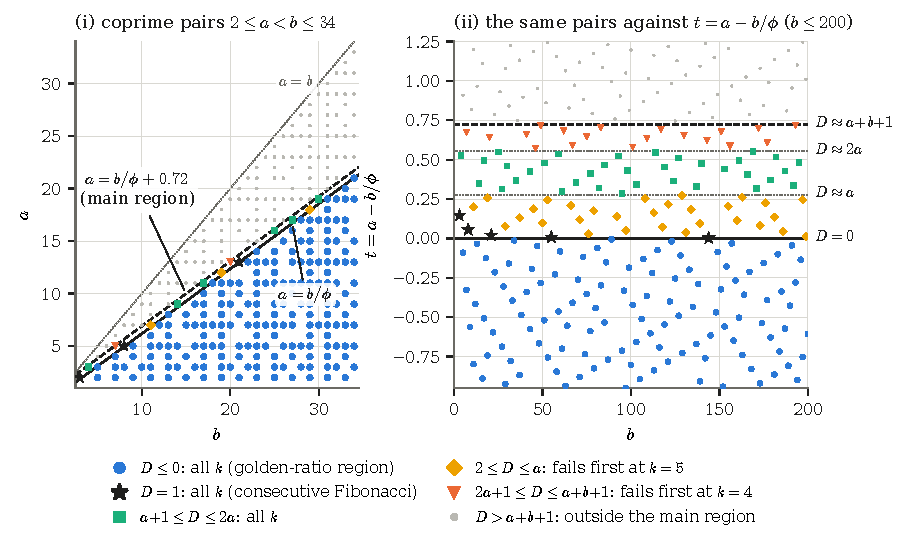
\includegraphics[width=\textwidth]{fig_golden.pdf}
\caption{The classes of coprime pairs $2\le a<b$ by the norm $D=a^2+ab-b^2=\mathrm N(a+b\phi)$. (i)~In the $(b,a)$ plane the classes lie along the line $a=b/\phi$ (solid), and the main region ends at $a\approx b/\phi+0.72$ (dashed). (ii)~Plotted against $t=a-b/\phi=D/(a+b\phi)$ the same classes become horizontal bands, with boundaries near $t=0$, $1/(\phi\sqrt5)\approx0.276$, $2/(\phi\sqrt5)\approx0.553$ and $\phi/\sqrt5\approx0.724$ (Table above). ``All $k$'' means that condition (I2) holds at every step, so $\R_k\ge L_k$ for every $k$ (Theorem~\ref{thm:D}); the consecutive Fibonacci pairs ($D=1$, stars) are the exception that lies inside the band of the class $2\le D\le a$.}
\label{fig:golden}
\end{figure}
\paragraph{Why a norm?} In every proof above, $D$ enters through one comparison: the largest ``dangerous'' sum $am+bs$ is about $(a+b)\cdot a\,L_{k-2}$, because the colour-$1$ numbers of $T_{k-1}$ reach up to $a/b$ of the length $L_{k-1}\approx bL_{k-2}$, while the forbidden window starts at about $b^2L_{k-2}$. So everything hinges on the sign and size of $a(a+b)-b^2=D$, a binary quadratic form of discriminant $5$. All forms of discriminant $5$ are equivalent to $x^2+xy-y^2$ (the class number is $1$), and this form is the norm form of $\mathbb Z[\phi]$; this is why $\phi$ appears. The finer thresholds $a+1$, $2a$, $a+b+1$ come from the lower-order terms ($+2a$, $+a$) in $L_k$ and $M_k$.

\paragraph{Orbits.} Multiplication by the unit $\phi^2$ maps $a+b\phi$ to $(a+b)+(a+2b)\phi$. Hence
\[
  (a,b)\ \longmapsto\ (a+b,\ a+2b)
\]
preserves $D$ and $\gcd(a,b)$, multiplies $t$ by $\phi^{-2}\approx0.382$, and maps the main region into itself. Every pair with a given $D$ lies on an orbit of this map; for example $D=1$ gives the consecutive Fibonacci numbers $(2,3)\mapsto(5,8)\mapsto(13,21)\mapsto\cdots$, and $D=5$ gives $(3,4)\mapsto(7,11)\mapsto(18,29)\mapsto(47,76)\mapsto\cdots$.
\begin{proposition}\label{prop:orbit}
Let $D\ge2$. On each orbit, at most one main-region pair has (I2) failing first at $k=4$, at most one pair has (I2) at every step, and all further pairs have (I2) failing first at $k=5$. For $D=1$ every pair on the orbit has (I2) at every step.
\end{proposition}
\begin{proof}
Along an orbit $D$ is fixed and $a$ more than doubles in each step ($a+b>2a$). By Theorem~\ref{thm:D} the pair works for all $k$ iff $D/2\le a\le D-1$, an interval whose endpoints have ratio less than $2$; it fails first at $k=4$ iff $a\le(D-1)/2$ together with the main-region condition $D\le a+b+1<3a+1$, i.e.\ $a\in((D-1)/3,(D-1)/2]$, again a ratio less than $2$; and it fails first at $k=5$ iff $a\ge D$, which persists once reached.
\end{proof}
For example, on the orbit of $(3,4)$ the recursion works for all $k$ at $(3,4)$ only, and on the orbit of $(5,7)$ it fails at $k=4$ for $(5,7)$ and at $k=5$ for $(12,19),(31,50),\dots$ So, with the exception of the Fibonacci pairs, the recursion works for all $k$ only for pairs that are ``early'' on their orbit.

%======================================================================
\clearpage
\section{A small set for computer proofs of upper bounds}\label{sec:small}
%======================================================================
\begin{lemma}\label{lem:small}
Let $K,n\ge1$ and
\[
  S=\{\,am\le n:\ m\le K\,\}\ \cup\ \{\,x\le n:\ x\equiv n\pmod b\,\}.
\]
If $S$ has no $k$-colouring without monochromatic solutions inside $S$, then $\R_k(a,b)\le n$. The smallest element of $S$ may be given colour $0$.
\end{lemma}
\begin{proof}
A good colouring of $[n]$ restricts to a good colouring of $S$; renaming colours is harmless.
\end{proof}
For three colours we take $K=\R_2=b^2+b+1$. The resulting formula is about $25$ times smaller than the one for $[n]$. In all computed three-colour cases, the smallest $n$ for which $S$ is not colourable equals $\R_3$.

%======================================================================
\section{The family \texorpdfstring{$b=a+1$}{b=a+1}}\label{sec:j1}
%======================================================================
For $b=a+1$ and $a\ge7$ one checks that $m'=a^2+5a+8=a(a-3)+(a+1)\cdot8\in A$ and $am'=M+a-3$, hence $N=a^3+5a^2+8a$. Theorem~\ref{thm:lower} gives the lower bound.

\paragraph{Upper bound for $a\ge28$.} Following \cite[Lemma~4.5]{CDW22} we use numbers that are polynomials in $a$:
\[
  x_{q,r}=N-b(qa+r)\quad\text{(the residue class of $N$)},\qquad
  y_{q,r}=a(qb+r)\quad\text{(multiples of $a$)},
\]
with $q\in\{0,\dots,10\}\cup\{a-10,\dots,a+7\}$ (as polynomials) and $|r|\le12$. At $a=60$ we keep the $1236$ distinct polynomials whose values lie in $[1,N]$, and all solution triples among them. All $112{,}177$ triples are polynomial identities $a(x-y)=(a+1)z$, so they are solutions for every $a$. The resulting $3$-colouring formula ($337{,}768$ clauses; the number $a$ is coloured $0$) is unsatisfiable: CaDiCaL produced an LRAT proof, accepted by \texttt{lrat-check} and by the formally verified checker \texttt{cake\_lpr} \cite{THM21}. Bounds on the roots show that for every $a\ge28$ the $1236$ values lie in $[1,N]$ and are pairwise distinct. Hence for every $a\ge28$ the formula is a subformula of the colouring formula of $[N]$, and $\R_3\le N$. (An independent numerical check at $a=28,\dots,129$, $500$, $1000$ and $10^6$ found no error.)

\paragraph{Upper bound for $7\le a\le27$.} Lemma~\ref{lem:small} at $n=N$, with LRAT proofs checked by \texttt{cake\_lpr} (Section~\ref{sec:comp}). This proves Theorem~\ref{thm:j1}. For $a=2,\dots,6$ the values are $61$, $109$, $180$, $300$, $462$.

\begin{remark}
The same shape of family does not suffice for $b=a+2$: the minimal unsatisfiable cores contain numbers at positions near $a/2$, so a parametrisation by the parity of $a$ would be needed. A single family in two parameters for the whole main region fails, because the necessary set grows with $b/a$.
\end{remark}

%======================================================================
\clearpage
\section{The three-colour upper bound: reduction to one statement}\label{sec:upper}
%======================================================================

\subsection{Chain and copy}
Let $N=N(a,b)$, let $r\in[1,b]$ with $r\equiv N\pmod b$, and $T=(N-r)/b$. We use two parts of $[N]$:
\begin{itemize}
\item the \emph{chain} $\{r+bt:\ 0\le t\le T\}$, whose elements we call \emph{positions} $t$;
\item the \emph{copy} $a\cdot[1,\R_2]=\{am:\ 1\le m\le \R_2\}$.
\end{itemize}
For a colouring $\chi$ of $[N]$ put $\varphi(m)=\chi(am)$ and $\psi(t)=\chi(r+bt)$. Two positions $t<u$ with $s=u-t\le\R_2$ give the solution $(r+bu,\,r+bt,\,as)$, so
\begin{equation}\label{eq:chain}
  \psi(t)=\psi(u)=\varphi(u-t)\quad\text{is impossible}.
\end{equation}
A position whose number is $am$ with $m\le\R_2$ is called \emph{special}; there $\psi(t)=\varphi(m)$. The special positions form one residue class modulo $a$.
By computer, these constraints together with the solutions inside the copy are already contradictory at $N$ and satisfiable at $N-1$ (all main-region pairs with $b\le15$, and all other pairs with $b\le17$ and $a\nmid M$).

\begin{conjecture}[S]
Every good $3$-colouring of $[N-1]$ uses only two colours on $a\cdot[1,b(b+1)]$.
\end{conjecture}

We verified Conjecture~S by computer in the following forms:
\begin{itemize}
\item in the stronger form ``$\varphi(s)\ne\varphi(\R_2)$ for all $s<\R_2$'', for the system of chain and copy above (whose good colourings include the restrictions of good colourings of $[N-1]$), for all main-region pairs with $b\le9$ and several more pairs up to $(4,7)$;
\item in the weaker form needed in Lemma~\ref{lem:W} (ten specific elements of the copy have the pattern colours), for all main-region pairs with $4\le b\le30$ except $(2,5)$;
\item in the form ``lower part plus Theorem~\ref{thm:upind}'' of Section~\ref{sec:lowerpart}, for all main-region pairs with $b\le30$ except $(2,3)$ and $(2,5)$.
\end{itemize}
For $(2,3)$ and $(2,5)$ Conjecture~S is false, in agreement with $\R_3(2,3)=61>N=52$ and $\R_3(2,5)=181>N=176$. All these checks use a SAT solver without proof files.

\subsection{Proof of the reduction}
We say that the copy has the \emph{pattern} if, for three distinct colours $c_0,c_1,c_2$,
\[
  \varphi(m)=c_0\ \ (m\in\{a,2a,\dots,ab\}),\qquad
  \varphi(m)=c_1\ \ (\text{other } m\le b(b+1)),\qquad
  \varphi(\R_2)=c_2 .
\]

\begin{proof}[Proof of Theorem~\ref{thm:red}]
Let $\chi$ be a good colouring of $[N]$. Its restriction to $[N-1]$ is good, so by Conjecture~S the colouring $u\mapsto\chi(au)$ of $[b(b+1)]$ uses two colours. It has no monochromatic solution, because solutions inside the copy are $a$ times solutions in $[b(b+1)]$. By Theorem~\ref{thm:R2} it is the colouring with $Q$ in one colour $c_0$ and the rest in another colour $c_1$. By the last part of the proof of Theorem~\ref{thm:R2}, applied inside the copy, $\R_2$ can have neither colour, so $\varphi(\R_2)=c_2$. Thus the copy has the pattern, and Lemma~\ref{lem:W} (main region) or Lemma~\ref{lem:Wout} (otherwise) gives a contradiction.
\end{proof}

\begin{lemma}[main region]\label{lem:W}
Let $N=1+bT$ with $T=\R_2+2a$, and let the copy have the pattern. Then the seven positions
\[
  0,\ a,\ 2a,\ \R_2,\ \R_2+a,\ \R_2+2a\quad\text{and one special position $p$}
\]
cannot be coloured so that \eqref{eq:chain} holds.
\end{lemma}
\begin{proof}
\emph{Choice of $p$.} Let $t_0\in[1,a-1]$ with $1+bt_0\equiv0\pmod a$. Choose $p\in\{t_0+2a,\,t_0+3a\}$ such that $m=(1+bp)/a$ is not a multiple of $a$; this is possible because the two values of $m$ differ by $b$ and $a\nmid b$. Then $m<5b\le b(b+1)$, so $\psi(p)=\varphi(m)=c_1$.

\emph{No position has colour $c_1$.} The distances from $p$ to the six positions are
\[
  p,\ p-a,\ p-2a\qquad\text{and}\qquad \R_2-p,\ \R_2+a-p,\ \R_2+2a-p .
\]
The first three are $\equiv t_0\not\equiv0\pmod a$ and at most $4a$, so $\varphi=c_1$. The last three lie in $[1,b(b+1)]$ and are $\equiv\R_2-t_0\pmod a$. If $a\nmid\R_2-t_0$ they are not multiples of $a$, so $\varphi=c_1$. If $a\mid\R_2-t_0$ they are multiples of $a$ larger than $\R_2-t_0-3a$, which exceeds $ab$ whenever $b-a\ge4$; so again $\varphi=c_1$. (The finitely many main-region pairs with $b-a\le3$ have $a\le6$; these, and all pairs with $b\le300$, were checked by computer.) By \eqref{eq:chain} none of the six positions has colour $c_1$.

\emph{Counting.} Among $0,a,2a$ the distances are $a$ and $2a$, with $\varphi=c_0$; so at most one of them has colour $c_0$. The same holds for $\R_2,\R_2+a,\R_2+2a$. The three pairs $(0,\R_2)$, $(a,\R_2+a)$, $(2a,\R_2+2a)$ have distance $\R_2$, with $\varphi=c_2$; so each pair contains at most one position of colour $c_2$. Altogether at most $2+3=5$ of the six positions can be coloured. Contradiction.
\end{proof}

\begin{lemma}[outside the main region]\label{lem:Wout}
Let $a^2+(b-1)a>b^2+b+1$, $a\nmid M$ and $b\ge a+2$, so that $N=am'$ with $m'=au'+bu$. Let the copy have the pattern. Then the four positions
\[
  P_1=T-\R_2-a,\quad P_2=P_1+a,\quad P_3=T-a,\quad P_4=T
\]
and two special positions $Q_0,Q_1$ cannot be coloured so that \eqref{eq:chain} holds.
\end{lemma}
\begin{proof}
\emph{Preliminaries.} The number at $P_1$ is $N-b(\R_2+a)=N-M\in(0,ab]$, so $P_1\ge0$. Since $a\mid N$, the last position $T$ is special, and the special positions are those $\equiv T\pmod a$. Since $a\nmid M=b(\R_2+a)$ we have $a\nmid\R_2$, so $P_1$ and $P_2$ are not $\equiv T\pmod a$.

\emph{The position $Q_0$.} The number $a^2u'=N-abu$ lies in the chain, at position $Q_0=T-au$. It equals $a\cdot(au')$ with $u'\le b$, so $\psi(Q_0)=c_0$. Here $u\ge2$, because $u=1$ would give $am'\le a(ab+b)<M$. The distances $P_4-Q_0=au$ and $P_3-Q_0=a(u-1)$ have $\varphi=c_0$, so $P_3$ and $P_4$ do not have colour $c_0$.

\emph{The position $Q_1$.} Consecutive special positions carry numbers $am$ whose $m$ differ by $b$, and the numbers $a,2a,\dots,ab$ lie in distinct residue classes modulo $b$. So among the first two special positions after $P_2$ there is one, $Q_1$, whose number $am$ has $m\notin\{a,\dots,ab\}$. Its number is at most $ab+b(3a+1)$, so $m\le5b\le b(b+1)$ and $\psi(Q_1)=c_1$. The distances from $Q_1$ to $P_1,P_2$ are at most $3a+1$ and not multiples of $a$. The distances to $P_3,P_4$ are multiples of $a$ in $(ab,\,b(b+1)]$, because $Q_1>P_2$ and $T-a-Q_1\ge\R_2-3a-1>ab$ for $b\ge a+2$. So all four distances have $\varphi=c_1$, and no $P_i$ has colour $c_1$.

\emph{Conclusion.} Hence $P_3$ and $P_4$ both have colour $c_2$. The distance from $P_1$ to $P_3$ and from $P_2$ to $P_4$ is $\R_2$, with $\varphi=c_2$; so $P_1$ and $P_2$ both have colour $c_0$. But their distance is $a$, with $\varphi=c_0$. Contradiction.
\end{proof}

We checked by computer that $Q_0$ and $Q_1$ as described exist for all $10283$ pairs outside the main region with $b\le300$ and $a\nmid M$. The case $b=a+1$ is covered by Theorem~\ref{thm:j1} and, for $a\le27$, by computation. The $50$ pairs with $b\le300$ and $a\mid M$ (for example $(7,9)$ and $(13,16)$) need more of the copy; for them the chain-and-copy system is still contradictory at $N$ in all computed cases.

\begin{proposition}[the longest chain]\label{prop:chain}
In the main region, assume the copy has the pattern and $(a,b)\ne(2,3),(2,5)$ (and, for $b\le300$, the computer check in Lemma~\ref{lem:W}). Then the chain $\{1+bt:\ 0\le t\le L\}$, with its special positions coloured as the copy, can be coloured so that \eqref{eq:chain} holds if and only if $L\le\R_2+2a-1$.
\end{proposition}
\begin{proof}
For $L\ge\R_2+2a$ this is Lemma~\ref{lem:W}. For $L=\R_2+2a-1$, restrict the colouring of Theorem~\ref{thm:lower} of $[N-1]$ to the chain and the copy: on the copy it is the pattern (with $c_0,c_1,c_2$ the colours of $C_0,C_1,C_2$, since $a\R_2>ab(b+1)$), and the chain ends at $1+b(\R_2+2a-1)=N-b\le N-1$.
\end{proof}
So the term $+2a$ in $N=b(\R_2+2a)+1$ is exactly the length by which the chain can exceed the copy.

\subsection{Conjecture S follows from its lower part}\label{sec:lowerpart}
In this subsection $(a,b)$ lies in the main region, $T=\R_2+2a$, and we use only the chain positions $0\le t\le T-1$. Their numbers $1+bt$ are at most $N-b$, and the copy lies below $N$, so every good colouring of $[N-1]$ gives a colouring of the chain and the copy that satisfies \eqref{eq:chain} and has no monochromatic solution inside the copy. We call such a colouring of the chain and the copy \emph{admissible}. Let $P$ be the two-colour pattern on $[1,b(b+1)]$:
\[
  P(m)=c_0\ \ (m\in\{a,2a,\dots,ab\}),\qquad P(m)=c_1\ \ (\text{other }m\le b(b+1)).
\]
Conjecture~S says that $\varphi$ agrees with $P$ on $[1,b(b+1)]$ for some colours $c_0\ne c_1$ (by Theorem~\ref{thm:R2}, using only two colours there is the same as having this pattern).

\begin{lemma}\label{lem:A}
Every integer $m$ with $ab<m\le b(b+1)$ lies in $A=\{au'+bu:\ 1\le u,u'\le b\}$.
\end{lemma}
\begin{proof}
Let $u$ be the least positive integer with $bu\equiv m\pmod a$ and $bu\ge m-ab$. By minimality $b(u-a)<m-ab$, i.e.\ $bu<m$, so $u<m/b\le b+1$. Put $u'=(m-bu)/a$; this is an integer, $u'\ge1$ because $bu<m$, and $u'\le b$ because $m-bu\le ab$.
\end{proof}

\begin{theorem}[upper part]\label{thm:upind}
Let $K_0=\max(ab+4a,\,4b)$. If an admissible colouring has $\varphi=P$ on $[1,K_0]$, then $\varphi=P$ on $[1,b(b+1)]$.
\end{theorem}
\begin{proof}
We show $\varphi(m)=c_1$ for $m=K_0+1,\dots,b(b+1)$ in turn, assuming $\varphi=P$ on $[1,m-1]$. Since $m>ab$, $P(m)=c_1$.

\emph{$\varphi(m)\ne c_0$.} By Lemma~\ref{lem:A}, $m=au'+bu$ with $1\le u,u'\le b$. Then $(m,au',au)$ is a solution inside $[1,\R_2]$, so $(am,a\cdot au',a\cdot au)$ is a solution inside the copy. As $au',au\le ab<m$, both have colour $c_0$; so $\varphi(m)\ne c_0$.

\emph{$\varphi(m)$ is not a third colour.} Suppose $\varphi(m)=c_2\notin\{c_0,c_1\}$. Consider the six positions $0,a,2a,m,m+a,m+2a$; they lie in the chain since $m+2a\le b(b+1)+2a=T-1$. As in the proof of Lemma~\ref{lem:W}, let $t_0\in[1,a-1]$ with $a\mid 1+bt_0$, and choose $p\in[2a+1,4a]$ with $p\equiv t_0\pmod a$ such that $m_p=(1+bp)/a$ is not a multiple of $a$ (of the two candidates in $[2a+1,4a]$, the values of $m_p$ differ by $b$, so at most one is a multiple of $a$). Then $m_p\le(1+4ab)/a<4b+1$, so $m_p\le4b\le K_0<m$ and $\psi(p)=\varphi(m_p)=P(m_p)=c_1$.
The distances from $p$ to $0,a,2a$ are $p,p-a,p-2a\in[1,4a]$, all $\equiv t_0\not\equiv0\pmod a$, so $\varphi=c_1$ on them. The distances from $p$ to $m,m+a,m+2a$ lie in $[m-4a,\,m-1]$; those that are not multiples of $a$ have $\varphi=c_1$, and those that are multiples of $a$ are larger than $m-4a\ge K_0-4a+1>ab$, so again $\varphi=c_1$. By \eqref{eq:chain}, none of the six positions has colour $c_1$.
The distances $a$ and $2a$ have $\varphi=c_0$, so at most one of $0,a,2a$ has colour $c_0$, and at most one of $m,m+a,m+2a$. Hence at least two of $0,a,2a$ and at least two of $m,m+a,m+2a$ have colour $c_2$, and for some $i\in\{0,1,2\}$ both $ia$ and $m+ia$ have colour $c_2$. Their distance is $m$, with $\varphi(m)=c_2$, contradicting \eqref{eq:chain}.
\end{proof}

So Conjecture~S holds for $(a,b)$ as soon as the following \emph{lower part} holds: every admissible colouring has $\varphi=P$ on $[1,K_0]$ for some colours $c_0\ne c_1$. Since $K_0\approx ab$, the lower part concerns roughly the first $1/b$ of the copy. We do not have a proof of the lower part. We checked it by computer (CaDiCaL, without proof files) for all $156$ main-region pairs with $b\le30$, in two parts.
\begin{enumerate}[label=(\roman*)]
\item \emph{Start.} $\varphi(1)=\dots=\varphi(a-1)\ne\varphi(a)$. This holds for all pairs except $(2,3)$ and $(2,5)$. For $(2,5)$, for example, a good colouring of $[180]$ (which exists since $\R_3(2,5)=181$) has $\varphi(1)=\dots=\varphi(5)$.
\item \emph{Steps.} For $m=a+1,\dots,K_0$: if $\varphi=P$ on $[1,m-1]$, then $\varphi(m)=P(m)$. This holds for all pairs except $(2,3)$, where it fails at $m=5$.
\end{enumerate}
Together with Theorem~\ref{thm:upind}, Conjecture~S holds in the chain-and-copy form for all main-region pairs with $b\le30$ except $(2,3)$ and $(2,5)$. This gives no new values (for $b\le60$ the values are proved in Section~\ref{sec:comp}), but it shows that Conjecture~S is really a statement about the first $\max(ab+4a,4b)$ elements of the copy.

We record what the computation says about the steps, as a guide for a proof. Most steps are already contradictory using the copy alone, or using a configuration as in Lemma~\ref{lem:W} (six positions and one special position, possibly shifted by $q\in\{1,2\}$). The remaining $15845$ steps (in total over all pairs) need the whole chain, and they are of three kinds:
\begin{itemize}
\item excluding $c_0$ at a number $m\notin A$ (such $m$ are at most $ab$ by Lemma~\ref{lem:A}; examples are the multiples $jb$ with $j<a$);
\item excluding the third colour at small $m$; all these steps have $m<4b$, that is, they lie exactly below the range where the argument of Theorem~\ref{thm:upind} applies;
\item excluding $c_1$ at $m=au$ with $u$ close to $b$.
\end{itemize}
In these steps the contradiction comes from solutions that use elements of the copy larger than $m$, so the lower part does not seem to follow from a step-by-step induction. It looks more like a global uniqueness statement of the kind proved in Theorem~\ref{thm:R2}. We also observed that, assuming $\varphi(1)\ne\varphi(a)$, the chain positions $0,\dots,L-1$ with $L=b^2+2a+2=T-(b-1)$ already force the lower part, and no shorter chain does, for $151$ of the $155$ pairs other than $(2,3)$ (the exceptions are $(3,4)$, $(2,5)$, $(3,5)$, $(5,7)$, with shorter chains). We have no explanation of this length.

\subsection{Remarks on Conjecture S}
\begin{enumerate}[label=(\roman*)]
\item If the chain is shortened by $j\le a$ positions, exactly the top $j$ elements of the copy can leave the pattern (computed for main-region pairs with $b\le15$, with two exceptions).
\item The special positions carry one residue class of the copy, at spacing $a$. The counting argument in the proof of Theorem~\ref{thm:R2} (in every class one colour is ``tight'') is the natural tool, but with three colours the count has slack.
\item Once the copy is fixed, \eqref{eq:chain} is a colouring problem on an interval of integers in which colour $c$ must avoid the set of distances $\varphi^{-1}(c)$. With the same forbidden set for every colour this would be the colouring of a distance graph $G(\mathbb Z,D)$; with colour-dependent sets it is close to the $S$-packing colourings of distance graphs studied, e.g., in \cite{BFK20}, where colour $i$ must avoid all distances $\le s_i$. Colourings in which each colour has its own set of forbidden distances were introduced by Greenwell and Johnson \cite{GJ92} and are surveyed by Abrams \cite{Abr00} under the name ``upper chromatic number''; there the forbidden sets are small and the space is the line or $\mathbb Z$, while here the forbidden sets are large (they are given by $\varphi$) and the interval is finite. Lemmas~\ref{lem:W} and~\ref{lem:Wout} and Theorem~\ref{thm:upind} are small results of this type, and Conjecture~S might be approached from that side.
\end{enumerate}

%======================================================================
\clearpage
\section{Computations}\label{sec:comp}
%======================================================================
\begin{itemize}
\item \emph{Upper bounds with checked proofs, $b\le60$.} For every pair with $3\le b\le60$ and $\gcd(a,b)=1$ except $(2,3)$ ($1041$ pairs), the set of Lemma~\ref{lem:small} with $K=\R_2$ at $n=N(a,b)$ (at $n=181$ for $(2,5)$) was shown unsatisfiable by CaDiCaL with an LRAT proof. Every proof was checked by \texttt{lrat-check} and also by the formally verified checker \texttt{cake\_lpr} \cite{THM21} (all $1041$ proofs; the largest ones, $57\le b\le60$, with a heap of up to $14$\,GB). The pair $(59,60)$ is also covered by Theorem~\ref{thm:j1}, and $\R_3(2,3)=61$ is a small computation.
\item \emph{$b\le81$, all $1939$ pairs.} The same upper bounds by MiniSat (without proof files). No counterexample to Conjecture~\ref{conj:C3}.
\item \emph{Lower bounds.} The colourings of Theorem~\ref{thm:lower} and Lemma~\ref{lem:step} were also checked against all solutions by an independent program: for all $326$ pairs with $b\le34$ ($k=3$), and for $k=4,5$ in the cases mentioned in Section~\ref{sec:rec}.
\item \emph{Theorem~\ref{thm:D}.} Exact computation of (I2) via \eqref{eq:recsets}.
\item \emph{Conjecture~S.} The checks of Section~\ref{sec:upper} were made with CaDiCaL, without proof files.
\end{itemize}
\paragraph{Computing environment.} Almost all computations ran on one desktop PC; a few small ones (the checks of Section~\ref{sec:lowerpart}, item~(i), and some searches for colourings) ran in a Linux cloud sandbox with two cores.
\begin{center}
\small
\renewcommand{\arraystretch}{1.12}
\begin{tabular}{>{\raggedright}p{3.6cm}>{\raggedright\arraybackslash}p{10cm}}
\toprule
CPU & Intel Core i5-11400F (6 cores, 12 threads)\\
Memory & 32\,GB DDR4\\
GPU & NVIDIA GeForce RTX 3060 (not used; the SAT solvers run on the CPU)\\
System & Windows~11 Home; solvers and proof checkers in WSL (Linux)\\
Workers & $11$ processes\\
SAT solvers & MiniSat~2.2 and CaDiCaL~1.5.3 through PySAT (searches); CaDiCaL~3.0.1 (static build, commit \texttt{c607304}) for all LRAT proofs\\
Proof checkers & \texttt{lrat-check} (drat-trim, commit \texttt{2e3b2dc}); \texttt{cake\_lpr} (commit \texttt{a36874a}), heap $0.7$, $4$ or $14$\,GB\\
\midrule
Three-colour proofs, $b\le60$ & $1041$ formulas with $1239$ to $21{,}254{,}243$ clauses; proofs $16.7$\,GB in total (written to a temporary folder and deleted after checking); about $51$ hours of task time in total (sum over the workers; approximate, because the runs were stopped and resumed several times)\\
\bottomrule
\end{tabular}
\end{center}
Every clause of every encoding is re-checked against the equation by an independent routine. Programs, results and colourings are available at \url{https://github.com/IchiTaku326/rado-ab}; the formula and LRAT proof for Theorem~\ref{thm:j1} are included, while the $1041$ proofs for $b\le60$ are not stored (they are large) but can be regenerated and checked with the published scripts.

%======================================================================
\clearpage
\section{Open problems}\label{sec:open}
%======================================================================
We list what we could not prove, in order of importance for this paper.
\begin{enumerate}
\item Prove the lower part of Conjecture~S (Section~\ref{sec:lowerpart}). By Theorems~\ref{thm:upind} and~\ref{thm:red} this would prove Conjecture~\ref{conj:C3} in the main region for $a\nmid M$, and in particular Conjecture~1.1 of \cite{AZB25}. At present the three-colour upper bound $\R_3\le N$ is proved only for $b=a+1$ (Theorem~\ref{thm:j1}) and by computation for $b\le60$.
\item Determine $\R_3$ for the pairs with $a\mid M$, and prove Conjecture~S outside the main region (Lemma~\ref{lem:Wout} assumes it).
\item Is $\R_k=L_k$ in the cases of Theorem~\ref{thm:D}? This holds for $(3,4)$ and $k=4$ \cite{Ich26b}.
\item Question~\ref{conj:growth}: is the growth exponential at all, and with which base? (For $a>b$ the five-colour data suggest a base larger than $a$.)
\item Explain why the norm form $D=\mathrm N(a+b\phi)$ of the golden-ratio field governs the colourings (Section~\ref{sec:norm}).
\end{enumerate}

\paragraph{Changes in version 2.} Only the paragraph ``Growth in $k$'' of Section~\ref{sec:rec} (the four-colour values for $(5,2)$, $(5,3)$ now have checked proofs, and the bound $\R_5(4(x-y)=3z)\ge1401$ is added) and the reference \cite{Ich26b} changed. All theorems and proofs are unchanged.

\section*{Acknowledgements and disclosure}
Programs, computation plans, parts of the proofs and parts of the text were developed with the help of an AI assistant (Claude, Anthropic). All proofs were checked by the author, and all computational claims can be reproduced with the published programs. The author is responsible for the content.

\clearpage
\begin{thebibliography}{99}
\bibitem{Abr00} A.~Abrams, Upper chromatic numbers: an update, \emph{Geombinatorics} \textbf{10} (2000), no.~1, 4--11; arXiv:2506.19126.
\bibitem{AZB25} T.~Ahmed, L.~Zaman, C.~Bright, Symbolic sets for proving bounds on Rado numbers, in: Proc.\ SC-Square 2025, CEUR Workshop Proceedings 4116 (2025); arXiv:2505.12085.
\bibitem{BFK20} B.~Bre\v{s}ar, J.~Ferme, K.~Kamenick\'a, $S$-packing colorings of distance graphs $G(\mathbb Z,\{2,t\})$, arXiv:2005.10491 (2020).
\bibitem{CDW22} Y.~Chang, J.\,A.~De Loera, W.\,J.~Wesley, Rado numbers and SAT computations, arXiv:2210.03262 (2022).
\bibitem{GMT12} W.~Gasarch, R.~Moriarty, N.~Tumma, New upper and lower bounds on the Rado numbers, arXiv:1206.4885 (2012).
\bibitem{GJ92} D.~Greenwell, P.\,D.~Johnson, Jr., Forbidding prescribed distances for designated colors, \emph{Geombinatorics} \textbf{2} (1992), no.~1, 13--16.
\bibitem{Ich26a} T.~Ichikawa, The four-colour Rado number of $2(x-y)=3z$ is $226$: a cube-and-conquer computation with checked DRAT proofs, preprint, Zenodo (2026), \url{https://doi.org/10.5281/zenodo.23582301}.
\bibitem{Ich26b} T.~Ichikawa, Four-colour Rado numbers of $a(x-y)=bz$: seven values with checked proofs, companion preprint, Zenodo (2026), version~2, \url{https://doi.org/10.5281/zenodo.23902620}.
\bibitem{Rado33} R.~Rado, Studien zur Kombinatorik, \emph{Math.\ Z.} \textbf{36} (1933), 424--470.
\bibitem{Ruz93} I.\,Z.~Ruzsa, Solving a linear equation in a set of integers~I, \emph{Acta Arith.} \textbf{65} (1993), 259--282.
\bibitem{San26} T.~Sanders, On Rado's single equation theorem, arXiv:2603.18179 (2026).
\bibitem{THM21} Y.\,K.~Tan, M.\,J.\,H.~Heule, M.\,O.~Myreen, cake\_lpr: verified propagation redundancy checking in CakeML, in: \emph{TACAS 2021}, LNCS 12652, 223--241.
\bibitem{Yao14} O.\,X.\,M.~Yao, A note on the two-color Rado numbers for $a(x-y)=bz$, \emph{Ars Combin.} \textbf{113} (2014), 473--476.
\end{thebibliography}
\end{document}
